\documentclass[11pt]{report}

\usepackage{framed}
\usepackage[margin=1.25in,top=0.85in]{geometry}
\usepackage{tikz}
\usepackage{tocloft}
\usepackage{xcolor}

\definecolor{darkgreen}{rgb}{0,0.35,0}
\definecolor{purplish}{rgb}{0.4,0,0.6}

\usepackage[letterpaper,breaklinks,bookmarks,plainpages=false,
   colorlinks,citecolor=darkgreen,linkcolor=purplish]{hyperref}

%%%%%%%%%%%%%%%%%%%%%%%%%%%%%%%%%%%%%%%%%%%%%%%%%%%%%%%%%%%%%%%%%%%%%%%%

\begin{document}
\pagestyle{headings}

%%%%%%%%%%%%%%%%%%%%%%%%%%%%%%%%%%%%%%%%%%%%%%%%%%%%%%%%%%%%%%%%%%%%%%%%

\thispagestyle{empty}
\begin{center}\LARGE

\vspace*{\fill}

\phantomsection\belowpdfbookmark{Title Page}{bkm:title}

{\Huge FontAnvil 0.1}

\vspace*{1.5in}


\includegraphics{anvil.pdf}

\vspace*{\fill}

\end{center}
\clearpage

%%%%%%%%%%%%%%%%%%%%%%%%%%%%%%%%%%%%%%%%%%%%%%%%%%%%%%%%%%%%%%%%%%%%%%%%

\thispagestyle{plain}
\vspace*{\fill}

\phantomsection\belowpdfbookmark{Copyright}{bkm:copyright}

\begin{minipage}{\linewidth}
\noindent
Visit the FontAnvil home page at
\url{http://tsukurimashou.sourceforge.jp/fontanvil.php}

\vspace*{1in}

FontAnvil user manual\\
Copyright \copyright\ 2014\quad Matthew Skala

\vspace{\baselineskip}

This document is free: you can redistribute it and/or modify
it under the terms of the GNU General Public License as published by
the Free Software Foundation, either version 3 of the License, or
(at your option) any later version.

\vspace{\baselineskip}

This document is distributed in the hope that it will be useful,
but WITHOUT ANY WARRANTY; without even the implied warranty of
MERCHANTABILITY or FITNESS FOR A PARTICULAR PURPOSE.  See the
GNU General Public License for more details.

\vspace{\baselineskip}

You should have received a copy of the GNU General Public License
along with this document.  If not, see \url{http://www.gnu.org/licenses/}.

\vspace*{0.75in}

\emph{The above license for the document itself notwithstanding,} the
FontAnvil software described in this document comprises the work of many
different copyright holders who have licensed their contributions under a
variety of terms.  The package as a whole is GPL, but some portions of it
are also available under less restrictive licenses.  See the ``Licensing''
chapter of this document for more information.

\vspace{\baselineskip}

Anvil clip-art by ``Gerald\_{}G,'' public domain.

\end{minipage}

\clearpage

%%%%%%%%%%%%%%%%%%%%%%%%%%%%%%%%%%%%%%%%%%%%%%%%%%%%%%%%%%%%%%%%%%%%%%%%

\phantomsection\belowpdfbookmark{Contents}{bkm:contents}
\renewcommand\contentsname{Contents}
\renewcommand{\cftbeforesubsecskip}{0pt}

\tableofcontents

\clearpage

%%%%%%%%%%%%%%%%%%%%%%%%%%%%%%%%%%%%%%%%%%%%%%%%%%%%%%%%%%%%%%%%%%%%%%%%

\chapter{Introduction}

FontAnvil is a script language interpreter for manipulating fonts. 
FontAnvil is substantially compatible with the PfaEdit/FontForge native
scripting language, but FontAnvil is intended for non-interactive use; for
instance, invocation from the build systems of font packages like
Tsukurimashou.  To better serve font package build systems in general and
Tsukurimashou in particular, FontAnvil has no GUI and, to a reasonable
extent, avoids dependencies on external packages.

There was a program called PfaEdit for editing fonts in Postscript ASCII
format (\texttt{.pfa} files).  PfaEdit development continued for many years,
it changed its name to FontForge, and it became the \emph{de facto} standard
font editing program in the free software community.  FontForge is still
under active development to this day.  The main focus of FontForge is on
interactive editing by GUI users, and the proportion of its code and
development effort dedicated to such users is large and growing.

PfaEdit had a scripting language, which as far as I know never had an
official name.  I will call it ``PE script'' in the interests of neutrality;
the traditional filename extension for files in this language is
\texttt{.pe}.  Development of PE script continued into the FontForge era. 
Many free font packages use PE scripts executed by FontForge to process font
files non-interactively in the context of a build system.  I myself maintain
the Tsukurimashou Project (\url{http://tsukurimashou.sourceforge.jp/}),
which processes fonts using PE scripts on a massive scale (thousands of
script invocations per build).

Attempting to use a large and steadily-growing GUI program as a
non-interactive script language interpreter is not always convenient.  The
many external libraries needed to build FontForge implicitly become
dependencies of any font package that needs FontForge for its build system;
and it is not easy to get users to install them all correctly just to build
a font package.  It is also hard to predict whether a given version of
FontForge will actually work for a given script: with GUI enhancements, and
even social network features, as the strategic priorities for FontForge
development, it is frequently the case that the stable and correct execution
of scripts is not at the top of the priority list, and bugs in script
processing are fixed late if at all.

There was a recent proposal to remove PE script from FontForge entirely,
which if adopted would be fatal to systems that depend on it, and not at all
adequately addressed by the concommitant proposal to encourage current PE
script users to ``upgrade'' to Python.  That particular proposal was not
immediately implemented, but it seems clear that the writing is on the wall
for continued FontForge support of PE script.  The mere \emph{risk} of
possibly losing PE scripting in up-to-date versions of widely-used Linux
distributions at some unspecified point in the future is a big problem for
the Tsukurimashou Project.  FontForge for all its good points can no longer
be thought of as a stable platform for non-interactive font manipulation;
its priorities are other things entirely.  But my own project absolutely
requires a stable platform for non-interactive font manipulation.  FontAnvil
is intended to fill the gap.

FontAnvil's development is driven by the needs of the Tsukurimashou Project,
but my hope is that it will also be useful to the many other projects
currently using PE scripts for non-interactive font processing.  I am also a
member of the FontForge development team, and I hope that FontAnvil's
existence will reduce the pressure on the FontForge team to continue
development of code that is outside most of the team's interests and
expertise.  Splitting the PE script interpreter into a standalone package
should be beneficial to almost everyone involved.

Some plans and goals for FontAnvil are:
\begin{itemize}
\item Whatever Tsukurimashou needs from a font manipulation script
  interpreter.
\item Return statements indented to the same level as the surrounding code.
\item A ``remove overlaps'' command that works.
\item No GUI, Python, or exotic dependencies.
\item No recursive Autotools.
\item Correct memory management.
\item Simple directory and linking structure (in particular, no
  unnecessary shared libraries).
\item Main code repository in Subversion.
\end{itemize}

FontAnvil's departure point from FontForge was at this tagged revision on
Github: \url{https://github.com/mskala/fontforge/releases/tag/fontanvil}. 
That is not a mainline FontForge revision; it was synthesized by merging the
mainline master as of roughly February 5, 2014 with a few patches from other
branches that were current as of the beginning of March.  From there I
copied the code into a private Subversion server (private because I don't
want to publish some intermediate revisions that lack proper copyright
notices) and ripped out most of the code that was not required by FontAnvil,
that being the majority of the package.  I simplified the structure of the
package and the build system along the way.  Removing the last traces of
dead code will be a long-term project.  The first public revision of
FontAnvil was added as a subdirectory to the Tsukurimashou Project's
Subversion server on March 4, 2014.  Future releases will be available through
Tsukurimashou's Web site.

Since FontAnvil and FontForge are free software under compatible license
terms and share many potential users and one developer, there is some
possibility for cross-pollination and sharing of code and ideas between the
two.  However, I do not think it is likely that I will spend much time
trying to import future development from FontForge into FontAnvil, nor that
the FontForge team will spend much time trying to import future development
from FontAnvil into FontForge.  Not much future development on either
project will be particularly relevant to the other.  The two projects have
different goals and policies and are likely to diverge.  However, since PE
script is mature and neither side is likely to drastically change the
language, I think it is likely that for the most part FontAnvil and
FontForge will be able to run each other's scripts for as long as FontForge
chooses to include a PE script interpreter.

Of all the parts of a forge, an anvil is simple,
an anvil is trustworthy, and most of all, \emph{an anvil is stable}.

\vspace{1cm}

\noindent
Matthew Skala\\
mskala@ansuz.sooke.bc.ca\\
\url{http://ansuz.sooke.bc.ca/}

\clearpage

%%%%%%%%%%%%%%%%%%%%%%%%%%%%%%%%%%%%%%%%%%%%%%%%%%%%%%%%%%%%%%%%%%%%%%%%

\chapter{Building FontAnvil}

There are no immediate plans to build binary distribution packages; to use
this code you will have to build it yourself from sources.

\section{Dependencies}

Building FontAnvil requires several libraries and other resources.  FIXME
they should be listed here.

Building from a version control checkout also requires recent Autotools.

\section{From a version control checkout}

FontAnvil is available by anonymous Subversion checkout from
\url{http://svn.sourceforge.jp/svnroot/tsukurimashou/trunk/fontanvil/}. 
That is the main public repository for FontAnvil source code, and checking
out from there is (at least for the moment, while the code is in flux) the
preferred way to obtain FontAnvil.  The Tsukurimashou repository as a whole
is also mirrored on Github at
\url{https://github.com/mskala/Tsukurimashou.git}, but Git unfortunately
does not offer any easy way to clone only the FontAnvil portion of the
repository.

The version control system does not track files that would be included in a
distribution tarball but can be built automatically from source files
already under version control, and ``configure'' is one such, so it is
necessary to create it before building.  This will require having recent GNU
Autotools on your system.

\begin{verbatim}
autoreconf
automake --add-missing
autoreconf
\end{verbatim}

All three steps are necessary:  the first autoreconf will fail, but creates
files needed by automake, which in turn creates files needed for autoreconf
to finish its work.  All these commands will probably give a lot of error
and warning messages.  Then you can build and install in the usual way:

\begin{verbatim}
./configure
make
# as root:
make install
\end{verbatim}

The configure script supports \texttt{-{}-help} and most of the usual
options.
Note that FontAnvil's configure is a work in progress and may not correctly
detect or handle some libraries that it should.  Also still to do is a nice
display at the end of the configure run showing what libraries were and were
not found.

The build system should automatically detect and use multiple cores on a
computer that has them.

\section{From a distribution package}

Distribution packages are available from the FontAnvil home page at
\url{http://tsukurimashou.sourceforge.jp/fontanvil.php}.

Building from one is much the same as building from a version control
checkout, minus the need to build \texttt{configure}.  Unpack the tarball
file and do the usual Autotools build:

\begin{verbatim}
./configure
make
# as root:
make install
\end{verbatim}

\section{FontAnvil and Tsukurimashou}

FontAnvil's reason for existence is to support Tsukurimashou, and its source
control repository is a subdirectory of the Tsukurimashou source control
repository, but FontAnvil is not a ``parasite'' of Tsukurimashou in the
technical sense of that term defined by the Tsukurimashou build system. 
Building Tsukurimashou will not automatically also build FontAnvil.
FontAnvil does not require Tsukurimashou to build.  (The very latest
development verion of) Tsukurimashou will look
for FontAnvil and use it if found, but will not look inside its own
subdirectories---only in the usual PATH search used for other utility
programs.  If Tsukurimashou does not find an executable in the search path
named ``fontanvil,'' it will fall back to looking for one called
``fontforge,'' just like earlier versions did.

If you want to use FontAnvil to build Tsukurimashou, you should build and
install FontAnvil first in the usual way, and then start building
Tsukurimashou.

All bug reports and other tickets for FontAnvil should be filed through
the Tsukurimashou ticket tracker at
\url{http://sourceforge.jp/projects/tsukurimashou/ticket/}.  Set the
``Component'' field to ``FontAnvil.''

As a courtesy to Github users, Tsukurimashou's entire source control system
(including FontAnvil) is mirrored in my Github account at
\url{https://github.com/mskala}.  But sourceforge.jp remains the
authoritative public home of the project.  You are welcome to clone the
repository---that is why it's there---but the semi-automated gateway from
Subversion to Git is one-way.  Do not file tickets for FontAnvil on Github.

\clearpage

%%%%%%%%%%%%%%%%%%%%%%%%%%%%%%%%%%%%%%%%%%%%%%%%%%%%%%%%%%%%%%%%%%%%%%%%

\chapter{Running FontAnvil}

FontAnvil is a script interpreter, so in normal operation it is assumed you
already have a script file for it to interpret.  Scripts are written in the
PE script language described elsewhere in this document.  Script files for
FontAnvil are traditionally given the filename extension \texttt{.pe} (for
``PfaEdit''); the extension \texttt{.ff} is also popular.  Invoking the
FontAnvil interpreter then proceeds on more or less the same lines as
invoking any other script interpreter.

\section{Command-line options}

\begin{framed}
FontAnvil's command-line syntax attempts to achieve some degree of FontForge
compatibility.  However, as of March~2014, FontForge contains at least six
different command-line
parsers,\footnote{https://github.com/fontforge/fontforge/issues/1277} and
also sometimes hands its command lines off to Python for parsing, so that
options interact in complicated ways with each other, with compile-time
settings, with operating system shebang support and whether stdin is a
terminal or pipe, and so on.  FontAnvil does not attempt to match all of
this behaviour exactly.
\end{framed}



FontAnvil uses GNU \texttt{getopt\_long\_only} to parse command-line
arguments; this has the consequence that long options may be specified with
\texttt{-} (one hyphen) or \texttt{-{}-} (two hyphens) as the flag sequence;
using \texttt{-{}-} is the modern-day Unix convention, but \texttt{-} may be
preferable for FontForge compatibility.  Short options require a single
hyphen.  Options recognized are as follows.

\begin{description}
  \item[\texttt{-command} $\langle cmd\rangle$,
    \texttt{-c} $\langle cmd\rangle$]
  Execute a PE script command given literally on the command line.  FontAnvil
  will \emph{not} look for a script file name on the command line if this
  option is specified; all arguments starting with the first non-option
  argument become arguments to the script.  Only the last invocation of this
  option will be used; unlike, for instance, Perl, it is not possible to
  build up a multi-line script by specifying \texttt{-c} multiple times.

  \item[\texttt{-dry}, \texttt{-d}]
  Activate a poorly-documented ``dry run mode'' built into some parts of
  the FontForge PE script interpreter.  This appears to
  be intended for syntax checking.  \emph{Most}, but not necessarily
  \emph{all}, commands will be skipped.  \emph{I do not promise that new
  code added in FontAnvil will necessarily respect this mode.}

  \item[\texttt{-help}, \texttt{-usage}, \texttt{-h}]
  Display a command-line option help message, and terminate without
  executing a script.

  \item[\texttt{-lang} $\langle cmd\rangle$,
    \texttt{-l} $\langle cmd\rangle$]
  Specify interpreter language.  If this option is given with the value
  ``\texttt{ff}'' then it will be ignored for compatibility.  Any other
  value is a fatal error.

  \item[\texttt{-nosplash}, \texttt{-quiet}, \texttt{-script}, \texttt{-i}]
  Ignored for compatibility.

  \item[\texttt{-version}, \texttt{-v}]
  Display a version and copyright banner, and terminate without executing a
  script.

  \item[\texttt{-{}-}]
  Terminate option scanning.  All subsequent arguments will be treated as
  ``non-option arguments'' (thus eligible to become script file names or
  script arguments) even if they resemble FontAnvil options.  This would be
  what you might use if for some reason you needed to execute a script file
  that was named exactly ``\texttt{-script}.''
\end{description}

The first non-option command line argument will be taken as the filename of
a script file to execute, unless the \texttt{-c} option or one of its
synonyms has overridden this behaviour.  If the filename so specified is a
single hyphen, or if there are no non-option command line arguments
at all, then FontAnvil will enter \emph{interactive mode}, reading
commands from standard input, as described later in this chapter.  Any
command line arguments after any script filename will be passed
into the script in the variables \texttt{\$1},
\texttt{\$2}, and so on---even in the cases of \texttt{-c} and interactive
mode.

\begin{framed}
Option scanning stops at the first non-option argument encountered, which
will usually be treated as the script filename.  Any arguments after that
become arguments to the script (passed in the variables \texttt{\$1},
\texttt{\$2}, etc.) and not options for the FontAnvil interpreter.  For this
reason, options \emph{must} precede the script file name on the FontAnvil
command line.  For maximum compatibility, the \texttt{-script} option should
be the last option if you use it at all, with the script file name in a
separate argument, not attached using \texttt{=}.
\end{framed}

\section{Shebang}

FontAnvil may be invoked using the shebang convention.  Place a line
something like ``\texttt{\#!/usr/local/bin/fontanvil}'' at the top of a
file, and make the file executable, to create a script that can be run like
any other program and will automatically use FontAnvil as the interpreter.

Details of shebang support vary depending on the operating system.  On most
systems, the shebang line must specify an absolute path, and the
\texttt{env} program may be used to search for a command name in the path to
avoid hardcoding the absolute location of the interpreter into a script. 
There are also special considerations applicable to the length of the
interpreter path, arguments specified in the shebang line, and so on. 

\emph{FontAnvil does not have any special support for shebang.}  In
particular, it does not scan the script to look for its own name in the
shebang line.  Since the shebang line by definition starts with the comment
character \texttt{\#}, it will be skipped as a comment.  FontAnvil just
takes the script file name as an argument from the operating system, and
(assuming the script name does not happen to be something weird that looks
like an option) executes it, with any remaining arguments becoming arguments
to the script.  This is normally the desired behaviour.  However, be aware
that it is a technical difference from FontForge, which attempts to
determine whether it was invoked via the shebang mechanism and do smart
things depending the answer, including working around operating systems that
support this feature only poorly.  FontForge may possibly \emph{require}
options in the shebang line in at least some cases, to select which
scripting language it will use.

If you try to specify command-line options in the shebang line, then
depending on your operating system's support it is possible that FontAnvil
will not see the options even though FontForge would.  Some operating
systems have unintuitive behaviour regarding options specified in the
shebang line; for instance, combining all options into a single string
passed as one argument instead of splitting them on spaces.  For this
reason, authorities on Unix often recommend against using options in the
shebang line at all; nonetheless, people continue doing it.

For maximum compatibility with both interpreters, I suggest writing shebang
lines in PE script files as you would write them for FontForge (including
mentioning the filename ``\texttt{fontforge}''), and then invoking FontAnvil
on the files by other means when desired.  That way, FontForge will see the
interpreter name and any options it wants, and FontAnvil will ignore them.

\section{Interactive mode and readline}

FontAnvil is intended primarily for non-interactive use.  However, if it is
invoked without a script file name, or with ``\texttt{-}'' (a single hyphen)
as the script file name, then it will enter a special \emph{interactive
mode}, where it reads commands from standard input and executes them
immediately, line by line, rather than reading from a script file.  This can
be convenient for one-off editing tasks and testing the syntax and behaviour
of script commands.

If FontAnvil was compiled with the GNU Readline library and detects that
standard input is a terminal, then interactive mode will also offer
command-line editing and history using Readline.  The usual Readline
keystrokes (such as up and down arrows to recall earlier-typed command
lines) become available in this mode, and there are some minor changes to
the output formatting (in particular, the display of a command prompt) to
make it friendlier for interactive users.

%%%%%%%%%%%%%%%%%%%%%%%%%%%%%%%%%%%%%%%%%%%%%%%%%%%%%%%%%%%%%%%%%%%%%%%%

\chapter{Data model}
\label{sec:data-model}

Very many difficulties users have with font editing (both scripted and
interactive) come from an incomplete understanding of the data model
involved: what entities exist in a font and a font editor and what
relationships those entities have with each other.  The distinction between
glyphs and characters seems to be an especially frequent cause of confusion. 
This chapter attempts to describe FontAnvil's data model in a way that will
be useful to script programmers.

\section{Fonts in memory}

Because PE script was originally designed for controlling a GUI font
editor, it treats fonts as documents to be opened and closed, much as
a GUI editor might.

At any given time there exists a global set of fonts that are \emph{open}. 
These are stored in RAM.  Open fonts are associated with filenames, even if
the filenames do not actually exist on disk; the interpreter will assign
temporary filenames (usually similar to ``\texttt{Untitled1.sfd}'') to fonts
that were created in memory and not loaded from files.  The filenames should
be unique (no more than one open font sharing a filename), and it's not easy
to create a situation where they are non-unique, but I suspect that having
distinct open fonts with duplicate filenames may be technically possible and
likely to trigger bugs if attempted.

The set of open fonts is technically a sequence (with a specific order), not
an unordered set, and the order is visible to scripts through the
\verb|$firstfont| and \verb|$nextfont| built-in variables, but this fact is
seldom important.

At most one of the open fonts may be the \emph{current font}.  This state is
global.  Most font-editing operations implicitly apply to the current font. 
The \texttt{Open()} built-in function sets the current font, but its exact
behaviour is context-sensitive.  If the specified filename is already an
open font, then \texttt{Open()} just sets the current font to that one.  If
the specified filename is \emph{not} already an open font, then
\texttt{Open()} loads it from disk, causing it to become an open font, before
setting the current font to that one.

When the interepreter starts up, the set of open fonts is empty and there is
no current font.  In this state, any operation that implicitly refers to the
current font will fail; scripts can only use a small subset of the language
to create or open a font make it current.  The \texttt{Close()} built-in
function removes the current font from the set of open fonts (without saving
it to disk---that must be done as a separate operation if saving is desired)
and places the interpreter back into the state of having no current font. 
Note that the existence of a no-font state is a difference between PE script
and the FontForge GUI.  The GUI insists on always having at least one open
font and always having a current font, enforcing this rule by automatically
loading fonts from earlier editing sessions, automatically creating a new
empty font if the load fails, choosing another open font to be current when
one is closed, and terminating the program when the last font is closed.

\section{Glyphs and slots}

Here are two pictures of Don Quixote.\footnote{Left: Gustave
Dor\'{e}, 1863.  Right: Honor\'{e} Daumier, 1868.}

\begin{center}

\includegraphics[width=1.5in]{quixote-dore.jpg}\qquad
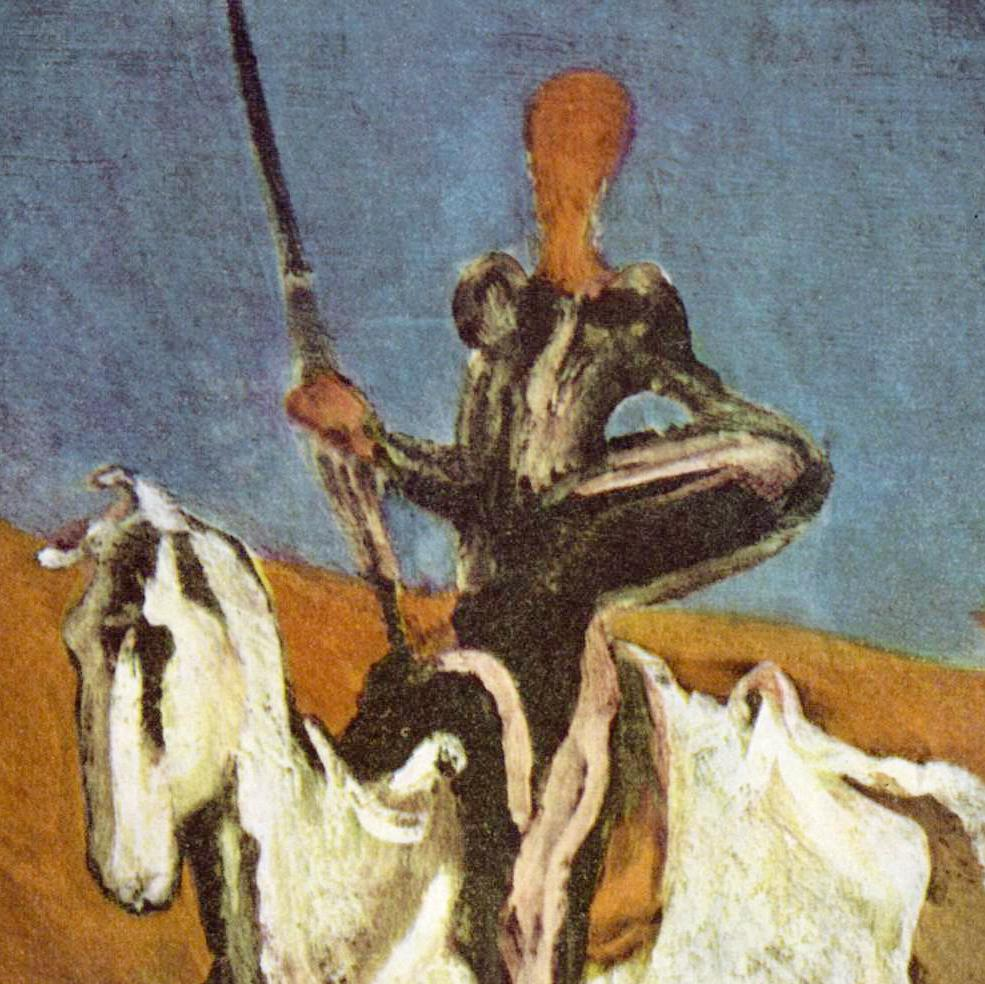
\includegraphics[width=1.5in]{quixote-daumier.jpg}
\end{center}

The pictures are different, but they are pictures of the same fictional
character.  In the same way, we can have several pictures of the same
character in a writing system.

\begin{center}
\scalebox{4}{a}\qquad
\scalebox{4}{\textit{a}}\qquad
\scalebox{4}{\texttt{a}}
\end{center}

What these three ``a''s share is the \emph{character}; what they do not
share is the \emph{glyph}.  Fonts contain collections of glyphs, concrete
things, which are pictures of characters, abstract things.  It is often the
case that in any given font, each glyph corresponds to exactly one character
and vice versa; but there are many important exceptions to that rule.  To
understand how FontAnvil processes fonts it is important to bear in mind
that fonts are collections of glyphs, and glyphs are not the same thing as
characters despite being closely connected with characters.

This glyph (the classic ff-ligature) is not associated with one character,
but with a sequence of two characters:

\begin{center}
\scalebox{5}{ff}
\end{center}

There is no double-f character, as a separate abstract entity distinct from
just two ordinary ``f''s in a row, in the English language.  There is no
standard character code for such a thing.\footnote{Actually, there is one in
Unicode, but you're not supposed to really use it; the details of that are
beyond the scope of this discussion.} Nonetheless a font for high-quality
typesetting of English must contain a glyph for this double-f entity
that is not quite a character.  Despite such exceptions, one glyph per
character is true most of the time in English.  In some other languages, the
conceit of glyph-character equivalence breaks down entirely.  In Arabic, for
example, many characters have four or more visual forms requiring
separate glyphs in a font, depending on how they connect to neighbouring
characters.

FontAnvil represents a font in memory as including a zero-based array of
\emph{glyph slots}.  The array is variable-sized, but it is a true array
data structure, not a list: all slots from index 0 up to one less than the
number of slots exist as long as the in-memory font does.  Creating a new
glyph means overwriting the possibly-blank previous contents of some slot. 
Destroying a glyph means filling the slot with a blank glyph, but the slot
continues to exist.  Changing the number of slots can only be done by
increasing or decreasing the length of the array, and encodings (described
in the next section) may constrain the number of slots.

Glyph slots in a font always have \emph{glyph numbers} which are their
indices in the array.  Glyphs in a font cannot meaningfully be said to be in
any specific order other than the order determined by the array indices. 
Every glyph has a number, and every number has a glyph slot.  No two glyphs
can have the same slot; two slots may contain identical glyphs, or even a
``reference'' from one to the other, but the two slots' contents will not
truly be the same entity.  A glyph slot might be \emph{blank}, that is
devoid of outlines and other data, and people usually think of such slots as
not really being glyphs.  But some attributes of a glyph slot (such as its
name) are required to always have non-null values, even on blank slots.

\begin{framed}
FontAnvil's in-memory glyph slots can be blank but never truly empty. 
However, most on-disk file formats \emph{do} have a concept of a glyph
failing to exist at all.  Blank slots are usually not written when saving
from memory to disk, and loading a file from disk to memory that does not
fill all slots will usually leave the others blank.
\end{framed}

Every open font has a \emph{selection}, which specifies a set of the glyph
slots (more about glyph slots in the next section).  Many editing operations
implicitly operate on the selection of the current font.  Although every
open font has a selection, usually only the selection of the current font is
relevant.  Open fonts retain their selections through changes in which open
font is current.

The selection is actually a sequence, not a set, of glyph slots.  That means
the slots in it can be selected in a specific order.  This distinction is
relevant in the FontForge GUI, where you can select several glyphs in a
specific order, open a ``Metrics'' window, and have them come up in the
order you selected them.  However, each glyph slot can appear at most once
in the selection, and the order of the selection is seldom if ever
observable or controllable from the scripting language.  It is usually
better to think of it as a set with no specific order, not as a sequence.

The selection is applied at the level of glyph slots.  It is perfectly
possible for the selection to include blank glyph slots, because it is
defined as a set of slots, not a set of non-blank glyphs.  Nonetheless, one
often only cares about the non-blank glyphs, and some commands for
manipulating the selection will automatically limit themselves to slots that
are not blank.

Glyph slot numbers \emph{may or may not} be closely connected to Unicode,
ASCII, or other character codes, depending on issues discussed in the next
section.  It is important to be aware that glyph slot numbers are not the
same type of entity as character codes, despite sometimes having equal
numerical values.

\section{Encodings}

Fonts do not exist solely to be edited with FontAnvil.  To be useful, a font
must eventually be saved in some format understandable by a word processor
or similar application; and the external software must be able to associate
the glyphs in the font with the characters in text that will be typeset
using the font.  There will necessarily exist some \emph{code} that
associates numbers called \emph{code points} with the different characters
that might appear in text, and a font file must explicitly or implicitly
describe which code points go with which glyphs.  It is worth emphasizing
that code points refer to characters, \emph{not glyphs}.

The ASCII code is familiar to many computer users, especially in the
English-speaking world, but is inadequate for languages other than English. 
Today, nearly everybody uses a code called Unicode.  Unicode's code points
coincide with ASCII for all the characters covered by ASCII; but it also
covers many thousands of other characters.  It is supposed to be a universal
code for all text in all human languages.  But Unicode did not always exist and its use was not always
universal.  Most common font formats are designed to also accomodate
character encoding schemes predating Unicode or simply other than Unicode. 
Frequently, a font file will include translation mappings for several
different codes, in the hope that software using the font can find its own
preferred code among the choices.  There needs to be a way to translate code
points (which identify characters) into glyph numbers (which identify
glyphs), even in cases like ligatures and variant glyphs where this
translation is more complicated than a simple one-to-one lookup.

FontAnvil includes several mechanisms for addressing these issues, but the
most significant is that of the \emph{encoding}.  The encoding is a
property of each font (global to the font) and describes a set of
assumptions and constraints about the relationships between code points and
glyph numbers.

\begin{framed}
Every glyph slot in a font always has a glyph number, no two slots can have
the same number, and the set of glyph numbers that exist is always the set
of integers from 0 up to one less than the number of glyphs in the font. 
Every code point designates at most one glyph slot.  But a glyph slot might
have zero, one, or more than one code point; a code point might have no
glyph slot; and the set of code points that exist might not be a simple
interval of the integers.  Nonetheless, the font's encoding may trigger the
enforcement of constraints that make the code point situation less
complicated.
\end{framed}

Most of the possible values of the encoding field are associated with
standardized character codes defined by external organizations.  Each code
defines a meaning for a range of code points from 0 up to some number that
depends on the code.  \emph{When the encoding is associated with an
externally standardized code other than Unicode}, FontAnvil enforces the
following constraints:
\begin{itemize}
\item There must be at least as many glyph slots as there are code points in
the code.
\item Glyph slots in the range 0 through one less than the number of code
points in the code correspond one-to-one with the code points.
\item Any glyph slots with greater indices have no code points.
\end{itemize}

The case of \emph{unencoded glyphs}, those in glyph slots beyond the end of
the code point range specified by the encoding, is important.  Glyphs like
the ff-ligature mentioned earlier, or the alternate forms of letters in a
script like Arabic, usually fall into this category.  When a word processor
typesets text using a font, it starts out by translating the code points
into glyphs one-for-one according to the basic code points of the glyph. 
The result of that translation cannot contain unencoded glyphs.  But the
basic one-for-one translation of code points to glyphs is only a starting
point.  Further processes can merge and split glyphs so that more than one
character can be typeset with one glyph, one character can be typeset with
more than one glyph, and which glyph goes with which character can be
different in different contexts.  These further processes can bring
unencoded glyphs into play.  The encoding does not specify the number of
unencoded glyph slots that may exist after the range of encoded glyphs.  The
unencoded glyph slots may be manipulated by built-in functions like
\texttt{SetCharCnt()}; encoded glyph slots may not be added or removed.

Each glyph slot has a property called the \emph{Unicode number}.  This is a
code point (in the code that is named Unicode), but I am going to call the
number in this field just a ``number'' to distinguish it from the code
points that exist in non-Unicode encodings.  When the encoding is one of the
standardized non-Unicode encodings, the constraint is enforced that the
Unicode number must be the correct translation (using the iconv library) of
the glyph number for encoded glyphs, or the null value of -1 for unencoded
glyphs.  For example, if the font's encoding is KOI8-R (commonly used for
Russian text), then glyph slot number 241 is for the letter ``ya,'' which
looks like a backwards R.  FontAnvil will enforce the constraint that this
slot's Unicode number is 0x042F, which is the Unicode code point for that
letter.  ``The constraint is enforced'' means that if you try to change the
value of the Unicode number field, the font's encoding will be immediately
changed to Custom.  Editing the Unicode numbers is not compatible with
keeping the encoding and its fixed mapping.

But not every value for the font's global encoding field is associated with
an external standard other than Unicode.  When the font's encoding field
refers to some form of Unicode, or does not refer to an external standard,
then additional special considerations apply; and in fact, these special
cases are the most popular and useful values for the encoding field.

When the encoding is set to Custom, few encoding-related constraints are
enforced.  There may be any number of glyph slots.  Any slot may have a
Unicode number, or not, and there is not necessarily any relationship
between the Unicode numbers and the glyph slots.

There are two Unicode encoding options, Unicode (BMP) and Unicode (Full). 
These each behave more or less like the non-Unicode standardized encodings. 
One difference is that it appears sometimes possible to set the Unicode
number of a glyph slot such that it does not match its glyph number.  This
may be a bug.  FIXME investigate further - this description may possibly be
simplified if Unicode and non-Unicode turn out to really behave the same.

FIXME investigate and document the ``Original'' encoding option.

Glyph slots have names.  All glyph slots have non-empty names, including
blank slots, and all names must be unique within a font.  The names are
sometimes automatically assigned and may also be manipulated by script
commands; but constraints (including the requirement for uniqueness) will be
enforced on such manipulation.

\begin{framed}
People who think they want to edit glyph slot names are often wrong.
\end{framed}

FIXME document name lists

\section{The \texttt{.notdef} glyph}

FIXME

\section{The clipboard}

There is a global entity called the \emph{clipboard}, which holds glyph data
of the kind that might be stored in glyph slots, such as outlines, anchors,
and references.  The clipboard is like a font in that it can store a bunch
of slots' worth of data, in a definite order, but the clipboard is unlike a
font in that the slots do not have meaningful numbers and it does not store
slot attributes other than glyph data, such as slot names and code points. 

The usual way of using the clipboard is somewhat like using the clipboard in
any common GUI document editor: select some slots, do a cut or copy
operation, select some other slots (even in a different font), and do a
paste operation.  Here is typical code to copy the uppercase ASCII alphabet
from an existing font into a new font (leaving many things in the new font
empty or default, which may cause problems later):

\begin{verbatim}
Open("font1.sfd");
Select('A','Z');
Copy();
New();
Select('A','Z');
Paste();
Save("font2.sfd");
\end{verbatim}

One thing to be aware of is that \texttt{Paste()} always writes into the
selection, and so you must create a nonempty selection for \texttt{Paste()}
to be meaningful.  This differs from a word processor that can ``insert''
text; FontAnvil treats a font as fixed framework of glyph slots that can
only be changed by overwriting.  Inserting or deleting in the middle, in a
way that changes the number of slots that exist, would disrupt the framework
of the encoding and is rarely, if ever, what you really want.

\begin{framed}
A glyph slot's name is associated with the glyph slot, not with the glyph
data stored in the slot.  The slot name will not move with the glyph data
when the glyph data is cut and pasted into a new slot.  Unicode code points,
and any other encoding numbers, are also parts of the glyph slot and will
not move with cut and pasted glyph data.
\end{framed}

\section{Look-up tables}

FIXME

\clearpage

%%%%%%%%%%%%%%%%%%%%%%%%%%%%%%%%%%%%%%%%%%%%%%%%%%%%%%%%%%%%%%%%%%%%%%%%

\chapter{Language reference}

\begin{framed}
I did not invent the PE scripting language, and the person who did never
fully specified or documented it.  This documentation is based partly on
reverse engineering; is descriptive, not prescriptive; and may not be
complete, nor even correct as far as it goes.  The only way to be sure
what a PE script will really do is to run it and find out, like
Rikki-Tikki-Tavi.
\end{framed}

\section{Basic syntax}

Scripts are text files.  The traditional filename extension is \texttt{.pe}~;
scripts in the wild have also been seen using a \texttt{.ff} extension.

Comments may be marked in any of these ways:
\begin{verbatim}
# hash for a shell-like comment to the end of the line

// two slashes for a C++-like comment to the end of the line

/*
C-style comment delimiters,
which may cover multiple lines.
*/
\end{verbatim}

FontForge looks for a shebang line at the top, pointing at itself, and may
also attempt to recognize command-line options there to distinguish between
PE scripts and Python scripts.  FontAnvil only supports PE scripts and is
planned to more or less ignore the shebang; however, this code has not yet
been worked over since its importation from FontForge and may not really
work as desired at the moment.

\begin{framed}
Newlines are syntactically significant, marking the ends of
statements.
To continue a statement onto more than one line, you must use a backslash to
escape the newline.  
\end{framed}

Semicolons also mark the ends of statements, and may be used to join
multiple statements onto a single line.  Semicolons at the ends of lines
create empty statements, which are ignored.

\begin{framed}
PE script is case sensitive for reserved words, variable names,
and built-in function names.
\end{framed}

\section{Data types, variables, and scope}

Values have associated types.  Variables can hold values of arbitrary type
and remember what type they are.  The types are:
\begin{itemize}
\item integer
\item floating-point number
\item Unicode code point (note that this is a distinct data type from
``integer'')
\item string
\item array
\end{itemize}

Syntax for constant values looks like this:
\begin{verbatim}
# integers in decimal, hexadecimal, or octal, using C syntax
123     # first digit nonzero means decimal
0x52    # first digits 0x means hex, this is 82 decimal
041     # first digit zero and not hex means octal, this is 33 decimal

# floating-point numbers indicated by the decimal point; note the decimal
# point is always . regardless of locale
123.45  # basic decimal float
4.9e5   # scientific notation, this is 490000

# Unicode code points are hexadecimal numbers marked by 0u
0u1f4a9 # everybody's favourite

# strings have single or double quotes
'Single'
"double"
"foo\bar" # \n for newline
# it is not clear what other escapes may exist

# array literals use square brackets and commas
[1,2,3,0uABC,'foo']
\end{verbatim}

\begin{framed}
Literal string constants in PE script syntax are limited to 256 characters. 
You can, however, construct longer strings with multiple literals and the
concatenation operator.
\end{framed}

\begin{framed}
The language seems intended to allow arrays to have more than one dimension
(i.e.\ each element of an array may itself be an array) but such arrays are
currently broken in both FontForge and FontAnvil, and usually cause the
interpreter to crash.  I hope to fix this bug in FontAnvil, but if I fix it
and FontForge doesn't, then any scripts that make use of multidimensional
arrays will be incompatible with FontForge.
\end{framed}

\section{Operators}

FIXME

\section{Control structures}

FIXME

\section{Most of the built-in functions}

FIXME

This section should document the functions.  For the moment, there is
only a list:

ATan2,
AddATT,
AddAccent,
AddAnchorClass,
AddAnchorPoint,
AddDHint,
AddExtrema,
AddHHint,
AddInstrs,
AddLookup,
AddLookupSubtable,
AddPosSub,
AddSizeFeature,
AddVHint,
ApplySubstitution,
Array,
AskUser,
AutoCounter,
AutoHint,
AutoInstr,
AutoKern,
AutoTrace,
AutoWidth,
Autotrace,
BitmapsAvail,
BitmapsRegen,
BuildAccented,
BuildComposit,
BuildComposite,
BuildDuplicate,
CIDChangeSubFont,
CIDFlatten,
CIDFlattenByCMap,
CIDSetFontNames,
CanonicalContours,
CanonicalStart,
Ceil,
CenterInWidth,
ChangePrivateEntry,
ChangeWeight,
CharCnt,
CharInfo,
CheckForAnchorClass,
Chr,
Clear,
ClearBackground,
ClearCharCounterMasks,
ClearGlyphCounterMasks,
ClearHints,
ClearInstrs,
ClearPrivateEntry,
ClearTable,
Close,
CompareFonts,
CompareGlyphs,
ControlAfmLigatureOutput,
ConvertByCMap,
ConvertToCID,
Copy,
CopyAnchors,
CopyFgToBg,
CopyGlyphFeatures,
CopyLBearing,
CopyRBearing,
CopyReference,
CopyUnlinked,
CopyVWidth,
CopyWidth,
CorrectDirection,
Cos,
Cut,
DebugCrashFontForge,
DefaultATT,
DefaultOtherSubrs,
DefaultRoundToGrid,
DefaultUseMyMetrics,
DetachAndRemoveGlyphs,
DetachGlyphs,
DontAutoHint,
DrawsSomething,
Error,
Exp,
ExpandStroke,
Export,
FileAccess,
FindIntersections,
FindOrAddCvtIndex,
Floor,
FontImage,
FontsInFile,
Generate,
GenerateFamily,
GenerateFeatureFile,
GetAnchorPoints,
GetCvtAt,
GetEnv,
GetFontBoundingBox,
GetLookupInfo,
GetLookupOfSubtable,
GetLookupSubtables,
GetLookups,
GetMaxpValue,
GetOS2Value,
GetPosSub,
GetPref,
GetPrivateEntry,
GetSubtableOfAnchorClass,
GetTTFName,
GetTeXParam,
GlyphInfo,
HFlip,
HasPreservedTable,
HasPrivateEntry,
Import,
InFont,
Inline,
Int,
InterpolateFonts,
IsAlNum,
IsAlpha,
IsDigit,
IsFinite,
IsHexDigit,
IsLower,
IsNan,
IsSpace,
IsUpper,
Italic,
Join,
LoadEncodingFile,
LoadNamelist,
LoadNamelistDir,
LoadPrefs,
LoadStringFromFile,
LoadTableFromFile,
Log,
LookupStoreLigatureInAfm,
MMAxisBounds,
MMAxisNames,
MMBlendToNewFont,
MMChangeInstance,
MMChangeWeight,
MMInstanceNames,
MMWeightedName,
MakeLine,
MergeFeature,
MergeFonts,
MergeKern,
MergeLookupSubtables,
MergeLookups,
Move,
MoveReference,
MultipleEncodingsToReferences,
NameFromUnicode,
NearlyHvCps,
NearlyHvLines,
NearlyLines,
New,
NonLinearTransform,
Open,
Ord,
Outline,
OverlapIntersect,
Paste,
PasteInto,
PasteWithOffset,
PositionReference,
PostNotice,
Pow,
PreloadCidmap,
Print,
PrintFont,
PrintSetup,
PrivateGuess,
PrivateToCvt,
Quit,
Rand,
ReadOtherSubrsFile,
Real,
Reencode,
RemoveATT,
RemoveAllKerns,
RemoveAllVKerns,
RemoveAnchorClass,
RemoveDetachedGlyphs,
RemoveLookup,
RemoveLookupSubtable,
RemoveOverlap,
RemovePosSub,
RemovePreservedTable,
RenameGlyphs,
ReplaceCharCounterMasks,
ReplaceCvtAt,
ReplaceGlyphCounterMasks,
ReplaceWithReference,
Revert,
RevertToBackup,
Rotate,
Round,
RoundToCluster,
RoundToInt,
SameGlyphAs,
Save,
SavePrefs,
SaveTableToFile,
Scale,
ScaleToEm,
Select,
SelectAll,
SelectAllInstancesOf,
SelectBitmap,
SelectByATT,
SelectByColor,
SelectByColour,
SelectByPosSub,
SelectChanged,
SelectFewer,
SelectFewerSingletons,
SelectGlyphsBoth,
SelectGlyphsReferences,
SelectGlyphsSplines,
SelectHintingNeeded,
SelectIf,
SelectInvert,
SelectMore,
SelectMoreIf,
SelectMoreSingletons,
SelectMoreSingletonsIf,
SelectNone,
SelectSingletons,
SelectSingletonsIf,
SelectWorthOutputting,
SetCharCnt,
SetCharColor,
SetCharComment,
SetCharCounterMask,
SetCharName,
SetFeatureList,
SetFondName,
SetFontHasVerticalMetrics,
SetFontNames,
SetFontOrder,
SetGasp,
SetGlyphChanged,
SetGlyphClass,
SetGlyphColor,
SetGlyphComment,
SetGlyphCounterMask,
SetGlyphName,
SetGlyphTeX,
SetItalicAngle,
SetKern,
SetLBearing,
SetMacStyle,
SetMaxpValue,
SetOS2Value,
SetPanose,
SetPref,
SetPrefs,
SetRBearing,
SetTTFName,
SetTeXParams,
SetUnicodeValue,
SetUniqueID,
SetVKern,
SetVWidth,
SetWidth,
Shadow,
Simplify,
Sin,
SizeOf,
Skew,
SmallCaps,
Sqrt,
StrJoin,
StrSplit,
Strcasecmp,
Strcasestr,
Strftime,
Strlen,
Strrstr,
Strskipint,
Strstr,
Strsub,
Strtod,
Strtol,
SubstitutionPoints,
Tan,
ToLower,
ToMirror,
ToString,
ToUpper,
Transform,
TypeOf,
UCodePoint,
Ucs4,
UnicodeAnnotationFromLib,
UnicodeBlockEndFromLib,
UnicodeBlockNameFromLib,
UnicodeBlockStartFromLib,
UnicodeFromName,
UnicodeNameFromLib,
UnicodeNamesListVersion,
UnlinkReference,
Utf8,
VFlip,
VKernFromHKern,
Validate,
Wireframe,
WorthOutputting,
WritePfm,
WriteStringToFile,
bAutoCounter,
bDontAutoHint,
bSubstitutionPoints

\section{Built-in functions in FontAnvil and not in FontForge }

No such functions at the moment.

\section{Built-in functions in FontForge and not in FontAnvil }

Because FontAnvil does not support plugins, these built-in functions have
been removed from the language:  LoadPlugin, LoadPluginDir.

\section{Other notes}

FIXME

\clearpage

%%%%%%%%%%%%%%%%%%%%%%%%%%%%%%%%%%%%%%%%%%%%%%%%%%%%%%%%%%%%%%%%%%%%%%%%
\iffalse
\chapter{SFD file format}

FIXME should have some more real information here instead of just
injunctions to the sinful.

\begin{framed}
I did not invent the SFD file format, and the person who did never fully
specified or documented it.  SFD is not a standardized format.  This
documentation is based partly on reverse engineering and it is descriptive,
not prescriptive.  That means if you create an SFD file with software other
than FontAnvil, you are not entitled to expect FontAnvil to read it,
\emph{not even if your file conforms to this documentation}; and that
applies to every piece of software that wrote the file as SFD,
not only the most recent one.  A problem was once observed in which
someone created a bad SFD file using homemade software, loaded it, saved
it, loaded it again, and it blew up after the second load because the data
really was invalid all along, but in a subtle way that survived
the first load/save pass.  The \emph{only}
supported way to create SFD files for FontAnvil to read is by writing them
originally with FontAnvil, using no data that ever passed through an SFD
file created by other software.  In particular, exchanging SFD files
between FontAnvil and FontForge, although I expect it will usually work,
is not supported.
\end{framed}

An SFD file is not a canonical form, in the sense of that term used by
mathematicians.  It is normal and expected that loading an SFD file and then
saving it may produce a file not byte-for-byte identical to the original. 
Loading and saving should identically preserve the  ``font,'' that is to
say the abstract entity consisting of glyph outlines associated to slot
numbers, named metadata strings, and so on; but many different SFD files can
realize any given font, and the only way to preserve a specific file
identically is to retain a copy outside FontAnvil.  This fact may have
implications for storing fonts in version control systems.  Note that few,
if any, other font file formats are canonical forms either.

FIXME

It should be obvious that the purpose of using UTF-7 encoding here is to
hide characters like newline (which would otherwise end the field) from the
parser, so it is absolutely necessary to encode such characters using the
Base64-style escape sequences of UTF-7 even if you think a string that left
these characters literal could also be syntactically valid UTF-7 under some
third-party definition of UTF-7.  Without the requirement for newlines to be
encoded there would be no way to distinguish a multi-line value that
happened to contain what looked like SFD field names, from a single-line
value followed by the rest of the file.  Exactly which characters must be
encoded for safe parsing is not defined beyond the general rule that
FontAnvil should read anything that FontAnvil wrote uninfluenced.  The
safest thing for other software to do is to put the entire field value in a
single Base64-style escape sequence whether it needs it or not.  (That is
what Tsukurimashou does.) Note that RFC-2152 does not require any specific
characters to ever be literal in UTF-7 (it at most \emph{allows} some
literal characters), and in any case RFC-2152 would not be authoritative
over the observed behaviour of the code.

The number of glyphs must meet the constraints of the font's encoding. 
FontAnvil checks, as does the latest FontForge; but some versions of
FontForge still in popular use do not, and may crash if this rule is not
observed.  See Section~\ref{sec:data-model} for more information about
encodings.

The order in which glyphs are stored in an SFD file is not significant, will
not in general be preserved through a load/save cycle, and will not affect
the order in which glyphs are stored when generating any non-SFD format,
such as TrueType.  Slot numbers, not the physical sequence of the records in
the file, define the significant ordering of glyphs in a font.

\clearpage
\fi
%%%%%%%%%%%%%%%%%%%%%%%%%%%%%%%%%%%%%%%%%%%%%%%%%%%%%%%%%%%%%%%%%%%%%%%%

\chapter{Licensing}

George Williams put most of his work on PfaEdit, and subsequently FontForge,
under licensing notices such as this one:

\begin{quotation}
Copyright \copyright\ [years] by George Williams

Redistribution and use in source and binary forms, with or without
modification, are permitted provided that the following conditions are met:

Redistributions of source code must retain the above copyright notice, this
list of conditions and the following disclaimer.

Redistributions in binary form must reproduce the above copyright notice,
this list of conditions and the following disclaimer in the documentation
and/or other materials provided with the distribution.

The name of the author may not be used to endorse or promote products
derived from this software without specific prior written permission.

THIS SOFTWARE IS PROVIDED BY THE AUTHOR ``AS IS'' AND ANY EXPRESS OR IMPLIED
WARRANTIES, INCLUDING, BUT NOT LIMITED TO, THE IMPLIED WARRANTIES OF
MERCHANTABILITY AND FITNESS FOR A PARTICULAR PURPOSE ARE DISCLAIMED.  IN NO
EVENT SHALL THE AUTHOR BE LIABLE FOR ANY DIRECT, INDIRECT, INCIDENTAL,
SPECIAL, EXEMPLARY, OR CONSEQUENTIAL DAMAGES (INCLUDING, BUT NOT LIMITED TO,
PROCUREMENT OF SUBSTITUTE GOODS OR SERVICES; LOSS OF USE, DATA, OR PROFITS;
OR BUSINESS INTERRUPTION) HOWEVER CAUSED AND ON ANY THEORY OF LIABILITY,
WHETHER IN CONTRACT, STRICT LIABILITY, OR TORT (INCLUDING NEGLIGENCE OR
OTHERWISE) ARISING IN ANY WAY OUT OF THE USE OF THIS SOFTWARE, EVEN IF
ADVISED OF THE POSSIBILITY OF SUCH DAMAGE.
\end{quotation}

That is what is commonly called a \emph{Three-Clause BSD License}.  There
were many subsequent contributors to the software (see the \texttt{AUTHORS}
file in the root of a distribution tarball or version control checkout) and
many of them were content to keep the same license terms in place, with or
without adding their own names and years to the copyright notice at the
top.

However, some contributors have placed additional restrictions on their
work, most notably \emph{GNU GPL3+} licenses like this one:

\begin{quotation}
Copyright \copyright\ [year] [contributor's name]

This program is free software: you can redistribute it and/or modify
it under the terms of the GNU General Public License as published by
the Free Software Foundation, either version 3 of the License, or
(at your option) any later version.

This program is distributed in the hope that it will be useful,
but WITHOUT ANY WARRANTY; without even the implied warranty of
MERCHANTABILITY or FITNESS FOR A PARTICULAR PURPOSE.  See the
GNU General Public License for more details.

You should have received a copy of the GNU General Public License
along with this program.  If not, see
\url{http://www.gnu.org/licenses/}.
\end{quotation}

The Free Software Foundation takes the position that the three-clause BSD
license is GPL-compatible,%
\footnote{\url{http://www.gnu.org/licenses/license-list.html\#ModifiedBSD}}
meaning that it is legally permissible for a package that is under GPL3+ as
a whole to include material that is under three-clause BSD.  The presence of
GPL3+ contributions, however, forces the package as a whole to be licensed
GPL3+.  That being the case, both FontForge and FontAnvil should be treated
as GPL3+, just with the awareness that some files may also be used
separately from the package under the less restrictive three-clause BSD
license.

It is the current practice of the FontForge project to encourage
contributors of new material to apply GPL3+ notices to any new files, but
retain the BSD notices on files that already have those.  There was an
incident in which someone tried to apply a patch someone else had written to
a currently BSD-licensed file in FontForge---with the patch to become
roughly 1/1000th of the file's total volume.  The author of the patch
demanded that the whole file should become GPL3+, overriding the BSD notice
on it and the apparent intentions of the previous contributors to that file. 
I would like to avoid such incidents.

A few files have other distribution terms.  In particular, some parts of the
build system have very permissive licenses.

FontForge attempts to maintain a list of all the licensing terms of all the
files in the project; but their list has never been up to date, cannot
reasonably be expected to ever be up to date nor to stay up to date even if
it ever is at one moment, currently contains incorrect information, and
seems unnecessary.  I do not propose to make such a list for FontAnvil.

The current licensing policy for FontAnvil is substantially the same as that
of FontForge:
\begin{itemize}
\item FontAnvil as a whole is covered by the GPL version 3, or any later
version.
\item Some files in FontAnvil are also available under less restrictive
licenses.  You must consult the notices in those files for details.
\item I will place GPL3+ notices on new files I create within FontAnvil,
and encourage others to do the same.
\item I will leave files with existing broader-than-GPL notices under their
existing notices (possibly adding my own name and year copyright lines), and
encourage others to do the same.
\item I will not accept contributions that entail drastic changes to the
licensing status of work done by persons other than the contributor, and I
will discourage the submission of such contributions.
\end{itemize}

Finally, note that although FontAnvil is associated with the Tsukurimashou
Project, its licensing is not identical to that of other things included in
the Tsukurimashou Project.
\clearpage

%%%%%%%%%%%%%%%%%%%%%%%%%%%%%%%%%%%%%%%%%%%%%%%%%%%%%%%%%%%%%%%%%%%%%%%%

\end{document}
